\documentclass[conference]{IEEEtran}
\IEEEoverridecommandlockouts
% The preceding line is only needed to identify funding in the first footnote. If that is unneeded, please comment it out.
\usepackage{cite}
\usepackage{amsmath,amssymb,amsfonts, esdiff, siunitx}
\usepackage{algorithm2e, algpseudocode}
\usepackage{float}
\usepackage{graphicx}
\usepackage{parskip}
\usepackage{textcomp}
\usepackage{wrapfig}
\usepackage{xcolor}
\def\BibTeX{{\rm B\kern-.05em{\sc i\kern-.025em b}\kern-.08em
    T\kern-.1667em\lower.7ex\hbox{E}\kern-.125emX}}
\begin{document}

\title{A ROS-Based Stereo Camera and LiDAR Fusion Approach to Obstacle Detection and Avoidance for Scaled Vehicles\\
% {\footnotesize \textsuperscript{*}Note: Sub-titles are not captured in Xplore and
% should not be used}
\thanks{This project is supported by the National Sciences and Engineering Research Council of Canada}
}

\author{\IEEEauthorblockN{1\textsuperscript{st} Neelkant Teeluckdharry}
\IEEEauthorblockA{\textit{Department of Electrical and Computer Engineering} \\%(of Aff.) \\
\textit{McMaster University}\\
Hamilton, Canada \\
teeluckn@mcmaster.ca} }
% \and
% \IEEEauthorblockN{2\textsuperscript{nd} Given Name Surname}
% \IEEEauthorblockA{\textit{dept. name of organization (of Aff.)} \\
% \textit{name of organization (of Aff.)}\\
% City, Country \\
% email address or ORCID}
% \and
% \IEEEauthorblockN{3\textsuperscript{rd} Given Name Surname}
% \IEEEauthorblockA{\textit{dept. name of organization (of Aff.)} \\
% \textit{name of organization (of Aff.)}\\
% City, Country \\
% email address or ORCID}
% \and
% \IEEEauthorblockN{4\textsuperscript{th} Given Name Surname}
% \IEEEauthorblockA{\textit{dept. name of organization (of Aff.)} \\
% \textit{name of organization (of Aff.)}\\
% City, Country \\
% email address or ORCID}
% \and
% \IEEEauthorblockN{5\textsuperscript{th} Given Name Surname}
% \IEEEauthorblockA{\textit{dept. name of organization (of Aff.)} \\
% \textit{name of organization (of Aff.)}\\
% City, Country \\
% email address or ORCID}
% \and
% \IEEEauthorblockN{6\textsuperscript{th} Given Name Surname}
% \IEEEauthorblockA{\textit{dept. name of organization (of Aff.)} \\
% \textit{name of organization (of Aff.)}\\
% City, Country \\
% email address or ORCID}
% }
%
\maketitle

\begin{abstract}
In this article, the McMaster Autonomous Electrified Vehicle (MacAEV), a small-scale 1:10 RC vehicle, is used to simulate manual and autonomous driving modes. Currently, the autonomous driving algorithm solves an optimization problem using integrated data from the onboard Intel RealSense Camera and SLAMTEK A2M8 RPLidar to navigate around detected obstacles. However, this approach is highly computationally expensive, and many embedded systems cannot perform these calculations fast enough to course correct and avoid a collision. To resolve this issue, this article proposes an optimized methodology leveraging a ROS 2 (Robot Operating System) package designed for real-time performance in C++. This efficiently resolves the optimization problem and enhances obstacle avoidance capabilities for the MacAEV. 

% This document is a model and instructions for \LaTeX.
% This and the IEEEtran.cls file define the components of your paper [title, text, heads, etc.]. *CRITICAL: Do Not Use Symbols, Special Characters, Footnotes, 
% or Math in Paper Title or Abstract.

% TODO:
% -Architecture of McMaster AEV Car. 


\end{abstract}

\begin{IEEEkeywords}
Autonomous Vehicles, Electrified Vehicles, Data Fusion, Model Predictive Control (MPC),
Intel RealSense Camera, SLAMTEK A2M8 RPLidar, ROS 2 (Robot Operating System), Embedded Systems,
Computational Efficiency, Obstacle Avoidance
\end{IEEEkeywords}

\section{Introduction}
% This document is a model and instructions for \LaTeX.
% Please observe the conference page limits. 


%Problem: 1:10 autonomous vehicles are difficult to design, as sensory units required for navigation are often prohibitively expensive.
%Solution: by leveraging sensor fusion, the macAEV car can sucessfully perform both obstacle avoidance and detection in real time using relatively inexpensive equipment. 

%----- Introduction Structure ----
%  Problem introduction
%   Maybe exagerate the need for this, explain that faulty algorithms could cost lives. 
%   a) P1: Researchers need ways to prototype  self-driving algorithms in low-risk settings. 
%   b) solution is 



% Autonomous driving has undergone substantial development over the past few decades, driven by researchers and industry partners alike. For local path-planning, vehicles leverage algorithms  designed specially for obstacle avoidance which utilize sensory modules to gain an understanding of the surrounding environment. However, the deployment of algorithm-based navigation on real vehicles is impeded by financial limitations due to the associated cost of sensors and vehicle parts. For this purpose, small-scale vehicle platforms have emerged as ideal choice for educational and research purposes. 

%more specific
Autonomous driving has undergone substantial development over the past few decades, driven by researchers and industry partners alike. However, the testing and development of self-driving algorithms on real vehicles is often impeded by the risk posed to human lives. As such, scaled vehicles have emerged as the most suitable alternative for autonomous driving research, permitting researchers to perform rigorous testing of novel algorithms in low-risk settings. 

%discuss levels of autonomy 

For local path-planning, scaled vehicles leverage algorithms designed for obstacle avoidance, utilizing sensory modules to first detect objects followed by a control strategy to navigate around them. Light Detection and Ranging (LiDAR), an active sensor, is commonly used as a sensory module for these tasks due to the relability of its point cloud data. LiDARs are classified as either 2D or 3D: 3D LiDARs emit multiple laser beams in three dimensional space, while in contrast, 2D LiDARs produces a single beam at a time and yield a plane scanning. These advanced scanning features of 3D LiDAR scanners can be prohibitively expensive, restricting some researchers from employing scaled vehicles to the field of autonomous driving.

In this paper, the McMaster Autonomous Electrified Vehicle (MacAEV), a scaled vehicle designed at McMaster University (shown in Figure 1), utilizes sensor fusion to detect and avoid obstacles in real-time along a corridor. It is equipped with both a depth camera and a 2D LiDAR, which are interfaced with an embeded computer through Robot Operating System 2 (ROS 2). The data sampled by both sensors is manipulated and fused in C++, and an optimization-based control algorithm, described in Section II, is applied to avoid the detected obstacles. 


% Together, these sensory modules form a less expensive alternative to a high resolution laser scanner, through a low computational expense approach to obstacle avoidance using sensor fusion. 

% Furthermore, the software architecture of the embedded system is developed using C++ in ROS 2, ensuring an optimized real-time performance. 

\begin{figure}
    \centering
    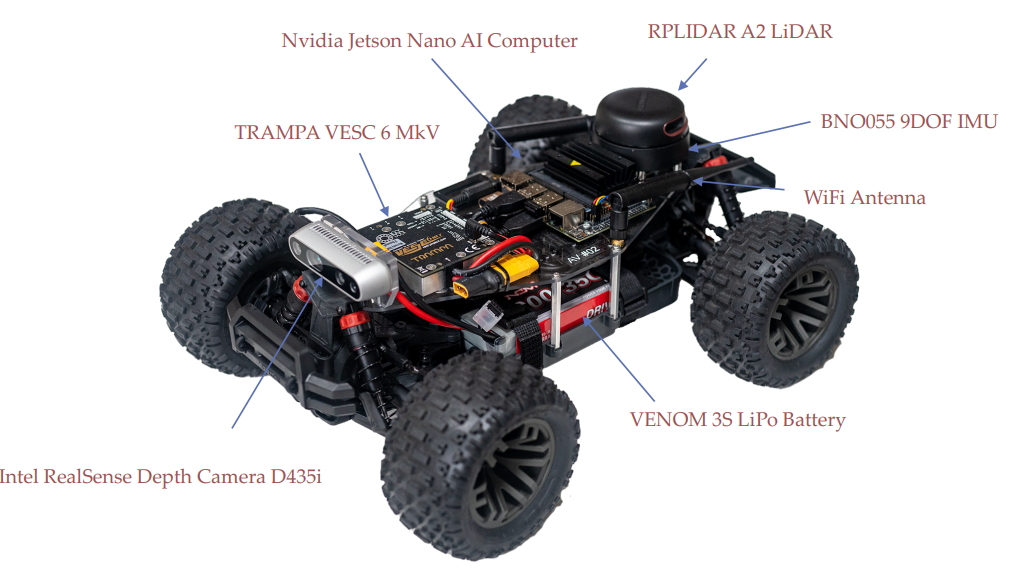
\includegraphics[scale=0.3]{vehicle.png}
    \caption{Shows hardware components of the MacAEV. \textbf{Image Credits:} Electrical Systems Integration Project Course.}
    \label{Figure 1}
\end{figure}

% Robot Operating System  (ROS) is a free, open-source, multilingual middleware providing communication between the user, the computer's operating system, and external equipment which can include sensors, camera, and other hardware in a robotic system. It comprises of a collection of tools and libraries serving as a platform for developing and executing robot applications. At the core of ROS is the concept of a node, which is an individual process that performs a computation or task. Nodes communicate with one another via topics which are channels carrying specific messages. Nodes can either publish or subscribe to a topic, consequently forming a publisher-subscriber network of nodes and topics \cite{b1}. 

% There are two generations of ROS, namely ROS 1 and ROS 2. Some key differences between ROS 1 and ROS2 include network architecture, client libraries, platform support and network transport \cite{b2}.  To remain faithful to the current state of art in robotics, this paper utilizes ROS 2 as middleware. 

% ROS 2 software is organized into packages, which are built through \textit{ament\textunderscore cmake} system and use \textit{colcon} as build tool. Packages facilitates the decomposition of ROS-based applications into modular units, that are easily integrable into various robotic systems or applications. This modular approach enhances reusability and modularity across different contexts. Furthermore, packages in ROS 2 encourage a collaborate development environment where developers can share and leverage existing components, which accelerates the development of complex robotic systems involved in various tasks such as obstacle avoidance, path planning and car following.  

% Examples of commonly used CNN models include Adaptive Spatial Feature Fusion (ASFF), CenterNet, EfficientDet and You Only Look Once (YOLO).

The paper is structured as follows: Section II examines related work. Section III discusses the 
algorithms used to detect obstacles and the control strategy used to navigate around them. Section IV examines the hardware components of the MacAEV and interfacing them through ROS 2. Section V discusses the implementation details of the system with specific insights into the data fusion and ground plane filtering algorithms. Section VI demonstrates the experimental results, showing sucessful obstacle detection and avoidance and Section VII concludes the paper and presents future directions. 


  % Monocular vision image-based methods for small-scale cars can be further subcategorized into three types:  appearance-based, motion-based and depth-based. Appearance-based methods identify obstacles in the foreground based on visual appearance. Motion-based methods detect objects using motion vectors. Depth-based methods determine the spatial arrangement of objects by utilizing depth. 
\section{Related Work}
Obstacle avoidance, a basic task in self-driving, is the backbone of autonomous navigation. Approaches to this task evolved from the Bug Algorithm in favor of path planning algorithms such as A* or Dijkstra on a local cost map \cite{b1}. In recent times, strategies to this task have now adopted machine learning flavor, giving rise to the optimization-based and model predictive control algorithms.    
Moreover, a critical aspect of successful obstacle avoidance hinges on accurate detection, for which a myriad of sensors can be employed to continuously scan the surroundings and identify obstacles. The most commonly used sensors for detection are LiDAR and camera, giving rise to LiDAR-based and vision-based approaches respectively \cite{b2}. 

Vision-based approaches use either computer vision (CV) or machine learning, specifically Convolutional Neural Network (CNN)-based algorithms such as in \cite{b3}. In the context of small-scale autonomous driving, the primary limitation to this approach is the restricted awareness of the surroundings due to the narrow field of vision captured by the camera sampling data. On the other hand, 2D Lidar-based methods, such as the Follow the Gap Method Method described by Sezer et al. in \cite{b4}, analyze raw returns to detect obstacles. Yet, relying solely on data sampled from a single plane can lead to potential blind spots and missed obstacles. This paper overcomes the limitations of both approaches by proposing a methodology of fusing the data and improves on existing optimization-based control algorithms to navigate around the detected obstacles.

\section{Used Algorithms}
The algorithm used for autonomous navigation follow the pipeline shown in the Figure.   

\begin{figure}
    \centering
    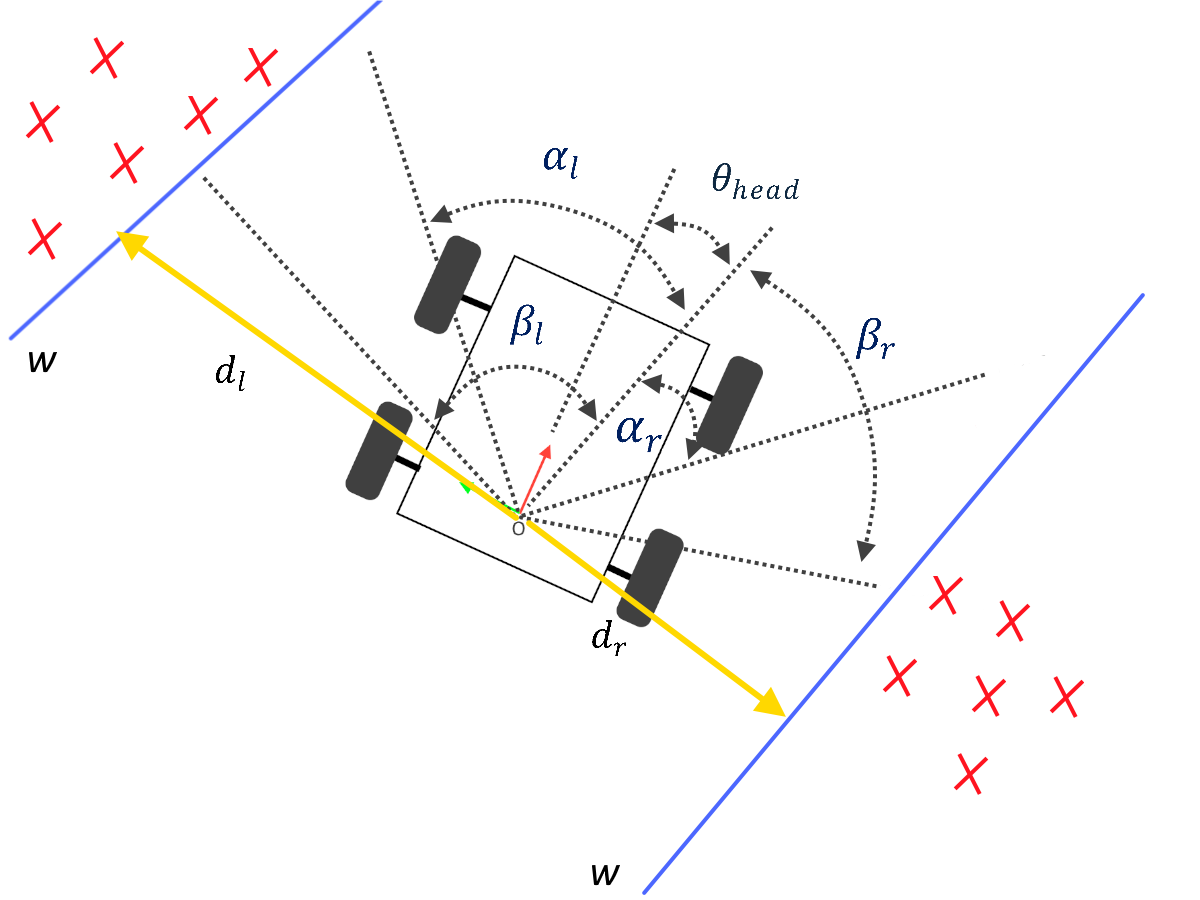
\includegraphics[scale=0.2]{diagram.png}
    \caption{Vehicle from top-view with labelled parameters used for retrieval of sensory information and control.}
    \label{Figure 3}
\end{figure}

\subsection{Calculating Heading Angle}

The LiDAR scans are captured and pre-processed as pairs $(\theta_i, r_i)$ of beam angles and corresponding range measurements. The scans are processed, assigning beam angles as increments of the LiDAR resolution with respect to the center of a predefined field of vision, namely $-\theta_{cen} \leq \theta \leq \theta_{cen}$ and ranges $0 \leq r_i \leq r_{max}$, where $r_{max}$ is the maximum LiDAR scan range. 

The heading angle, $\theta_{head}$, represents the desired direction of travel of the vehicle and acts as a reference to separate scans on the left and right sides of the vehicle in any orientation. It is calculated as a weighted average of beam angles based on the processed data:

\[\theta_{head} = \frac{\sum_{i} r_i \theta_i}{\sum_{i} r_i} \]

Two design parameters $\alpha_l$ and $\beta_l$, which are angles oriented on the left of $\theta_{head}$, are chosen.  The range measurements between these two angles are sampled and used to calculate the left barrier, as described in Section B below. Similarly, on the right side, $\alpha_r$ and $\beta_r$ are chosen, and the corresponding range measurements are used to calculate the right barrier. 

% As shown in Figure \ref{Figure 2}, the scans are sub-sampled between $\alpha_l$ and $\beta_l$, as well as $\alpha_r$ and $\beta_r$ which are used to form the left and right barriers respectively. The distance between the origin of the frame and the calculated walls is maximized based on these returns. 

\subsection{Finding the Barriers}
Suppose $w \in \Re^2$  is the vector which parametrizes the line separating the Lidar scans from the vehicle. The minimum distance, $d$, between the origin of the frame, centered at the Lidar, and the line is given by:

\begin{align}
    d = \frac{1}{w^T w} \notag
\end{align}

The lines on both sides of the vehicle are constrained to be parallel, to better fit the barriers. The goal is to find a vector $w$ which maximizes the total distance $d_{total}$, representing the total distance from the frame to the left barrier $d_l$ and frame to the right barrier $d_l$. 

\begin{align}
    d_{total} = d_l + d_r = \frac{2}{w^T w} \notag
\end{align}


This gives rise to a convex model predictive control problem with linear constraints or an inequality-constrained quadratic program.  

\begin{equation}
\begin{aligned}
        \min_{w}  \quad & J = \frac{1}{2}w^T w \\
        \text{s.t.} \quad & w^Tp_i + b - 1 \geq 0  \; \forall i \in \{1,...,n_l\} \\
        & w^Tp_j + b + 1 \leq 0 \; \forall j \in \{1,..,n_r\}\\ 
        & -1+\epsilon \leq b \leq 1 - \epsilon
\end{aligned}
\end{equation}


where $n_r$ and $n_l$ are the number of points sampled between $\alpha_r$ and $\beta_r$ and $\alpha_l$ and $\beta_l$ respectively. $b$ is a parameter representing the translation of the lines and $\epsilon > 0$.

The quadratic program is implemented in C++ by augmenting the vector $w$ with $b$ as a third component. This is accomplished by assigning a very small weight to $b$ in the positive semi-definite matrix $Q$ in $w^T Q w$, which represents the cost function $J$. The constraints are represented as linear combinations of $w_x, w_y$ and $b$, which are easily expressible in matrix form. Therefore, the dimension of the quadratic program is $n=3$, indicating it is  small-sized and can be feasibly solved on many embedded computers in real time. In the C++ implementation on the MacAEV, the Dual-Active Set Method proposed by Goldfarb and Idnani in \cite{b8} was used to compute the solution to the optimization problem, which demonstrated good real time performance. 
%%talk about what the solution to the program gives

%kinda bad
% In practice, solving this problem using a quadratic program solver requires defining vector $u = [x,y,b]$ and tailoring it further to the solver's required form. It can be shown that $w_l = \frac{u}{b+1}$ and $w_r = \frac{u}{b-1}$, which is a helpful result in the implementation. 

\subsection{Steering and Velocity Controller}
To drive the motor, the VESC controller is passed an \textit{ackermann\textunderscore msg} through ROS, which is a time-stamped message containing both the input velocity $v$ and steering angle $\delta$. The MacAEV acheives autonomy through precise control of $v$ and $\delta$ within a finite state-machine, where the behaviour of the vehicle changes in response to specific inputs like the detection of an obstacle in-front or behind. The MacAEV's state machine has three states: \textit{normal}, \textit{backup} and \textit{turn}. Developed in this section, are the associated calculations and behavioural descriptions of the vehicle within these states, each of which outputting a corresponding $v$ and $\delta$ as \textit{ackermann\textunderscore msg} to the VESC controller at every time step.  


In the \textit{normal} state, the vehicle slows down in the presence of detected obstacles and maintains an appropriate distance from the barriers. Thus, the control objective for steering is to control the distance $d_{lr} = d_l - d_r$ between the left and right barriers. These distances are represented in Figure 2. The non-linear dynamics of these distances are governed by these equations:


\begin{equation}
    \begin{aligned}
        \dot{d_{lr}} = -v_s \sin \alpha_l - v_s \sin \alpha_r
    \end{aligned}
\end{equation}  

\begin{equation}
    \begin{aligned}
        \ddot{d_{lr}} = -\frac{v_s^2}{l} (\cos \alpha_l + \cos \alpha_r)\tan \delta 
    \end{aligned}
\end{equation}

Equation (3) arises as a result of the bicycle kinematic model, used to derive the dynamics of the system. Moreover, the tracking error of $d_{lr}$ is minimized using a PD controller, the output of which is used to subsequently calculate the required steering angle $\delta$. 

\begin{equation}
        \delta_{lr} = \arctan \left( \frac{l ( k_p \Tilde{d_{lr}} +k_d \dot{d_{lr}} )}{v_s^2(\cos \alpha_{r} + \cos \alpha_{l} )} \right) 
\end{equation}




These distances can be expressed in terms of the horizontal components of the vectors found by solving the quadratic program in the previous section. Specifically, 


\begin{equation}
    \begin{aligned}
        \cos \alpha_l = \begin{bmatrix}
            0 & -1
        \end{bmatrix} \Vec{w_l} 
    \end{aligned}
\end{equation}

\begin{equation}
    \begin{aligned}
         \cos \alpha_r = \begin{bmatrix}
            0 & 1
        \end{bmatrix} \Vec{w_r}
    \end{aligned}
\end{equation}


Combining equations (4), (5) and (6) produces the closed form expression used in the implementation of the controller to find $\delta$.

\begin{equation}
    \begin{aligned}
        \delta_{lr} = \arctan \left( \frac{l(k_p \Tilde{d_{lr}}+ k_d \dot{d_{lr}})}{v_s^2(w_{ry} - w_{ly})} \right)
    \end{aligned}
\end{equation}

where $w_{ry}$ and $w_{ly}$ denote the y-component of the right and left wall vectors respectively.  



As previously stated, velocity is controlled based on distance to an incoming obstacle. This is given by:

\begin{equation}
    v = v_{s_0}\left[1-e^{-\max(d_{min}-d_{stop},0)}\right]
\end{equation}

where $v_{s_0}$ is the maximum vehicle velocity, $d_{min}$ is the minimum Lidar range reading, and $d_{stop}$ is the vehicle stop distance for an obstacle in front of it. It can analogously be seen as a potential field, where obstacles have a high potential and  the vehicle is repelled from them. If the velocity reaches below a defined threshold for a certain amount of time, it indicates that the vehicle has stopped, which triggers a state shift to \textit{backup}. 

The \textit{backup} state will cause the vehicle to move with the same velocity scale as in (8), however, in the opposite direction. There are two cases: either the pitch measured by odometry will indicate that the vehicle is oriented away from the closest obstacle or the vehicle will continue attempting to move backwards for a defined amount of time, after which the state will shift to \textit{turn} in both cases.

The \textit{turn} state is also defined with the same velocity scale as in (8). If the vehicle is already oriented away from the closest obstacle, then a state shift will be triggered to return to \textit{normal}. Otherwise, the steering angle will be set to maximum and if the vehicle is still unable orient itself away from obstacles, then it will return to the \textit{backup} state.

\section{System Design}




% \subsection{Convex Model-Predictive Control}
% The discrete linear quadratic regulator can be extended to include inequality constraints through convex model-predictive control (MPC). 

In this section, the hardware architecture and technical specifications of the MacAEV are presented.

\subsection{Hardware Architecture}

The McMaster AEV car, powered by a VENOM 3S lithium-polymer (LiPo) Battery, is built on an ARMA GRANITE 4x4 vehicle platform and consists of a multitude of sensors and actuators to interact with the environment. Central to these interactions are onboard computations handled by an Nvidia Jetson Orin Nano embedded computer. Some key features of this device include a microSD card slot, a 40-pin Expansion Header, 4x USB 3.2 Type A ports and a Display Port Output Connector \cite{b5}. The microSD card slot allows for Ubuntu 20.04 to be flashed onto the embedded computer through the Jetpack Software Development Kit 5 (Jetpack SDK 5). The USB Type A ports permit for sensors to be serially connected to the computer, which publish data through topics within the ROS 2 middleware. In this study, the data is manipulated within C++ nodes which are subscribed to the relevant topics. 

\begin{figure}
    \centering
    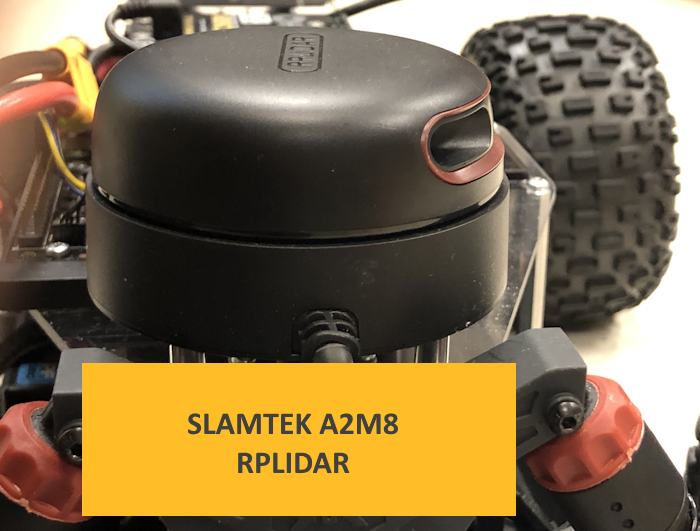
\includegraphics[scale=0.2]{lidar_diagram.png}
    \caption{Shows the SLAMTEK A2M8 attached on the vehicle extremity.}
    \label{Figure 2}
\end{figure}

The sensory modules on the MacAEV consists of a SLAMTEK A2M8 RPLIDAR, Intel RealSense Depth Camera D345, Adafruit BNO055 IMU and TRAMPA VESC MARK VI. Key features of the SLAMTEK A2M8 RPLIDAR (shown in Figure 2) include the use of TTL UART to communicate with the embedded computer, a sample rate of 8 kHz, an angular resolution of \ang{0.225} and serial baud rate of 115 200 bits per second. The RPLIDAR is connected to the Nvidia Jetson through a USB type A port and publishes both the angular heading and distance of captured point clouds \cite{b6}. Using the RPLidar in ROS 2 requires the installation of SLAMTEK's \textit{rplidar-ros2} package which allows a node capable publishing data to a topic called \textit{/scan} to be initialized.

\begin{figure}
    \centering
    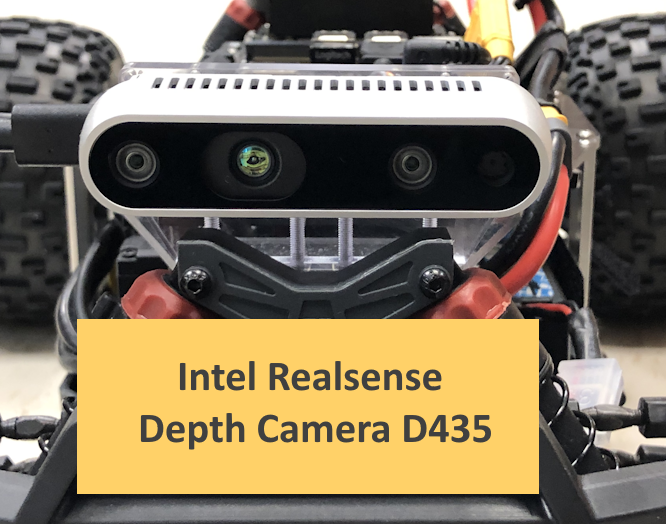
\includegraphics[scale=0.25]{realsense_diagram.png}
    \caption{Shows the Intel RealSense Depth Camera attached to the vehicle extremity.}
    \label{Figure 3}
\end{figure}


The Intel RealSense Depth Camera D345 shown in Figure 3 combines both RGB and infrared stereoscopic depth cameras with an inertial measurement unit (IMU). Within the camera, the stereo-depth module captures images at 90 frames per second at a resolution of 1280 by 720 pixels, using left and right imagers. Then, data is processed by the vision processor to correct the captured image. Finally, the processed data is stored in the camera's memory through an EEPROM \cite{b7}. Using the camera in ROS 2 requires the installation of the \textit{realsense-ros} package, which enables the use of the \textit{realsense2\textunderscore camera} node. This node publishes color, depth, extrinsic and inertial measurements across eight different topics. The algorithms used for autonomous navigation in this paper rely on depth imaging. 
% This camera is commonly used improve the environmental awareness of the MacAEV, permitting navigation in complex environments, the detection obstacles, and more efficient interactions with surroundings.

\begin{figure}
    \centering
    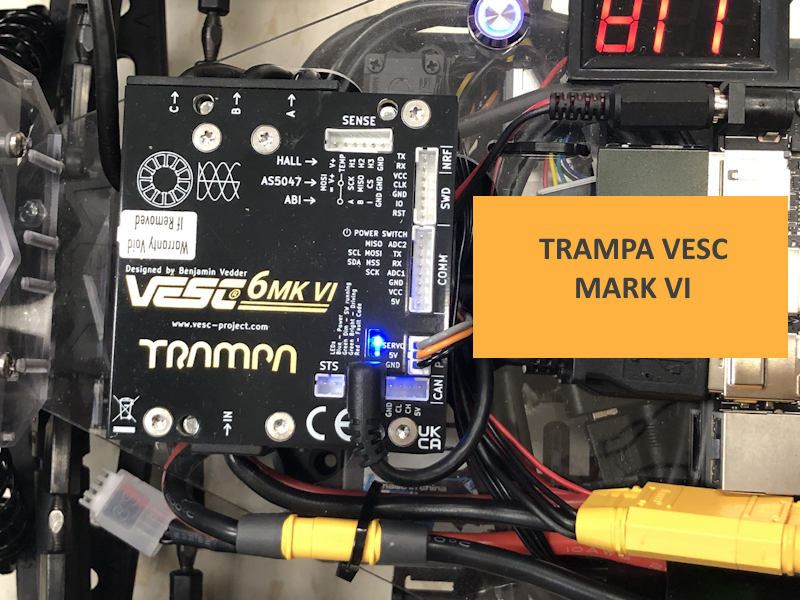
\includegraphics[scale=0.2]{motor_ctrl_diagram.png}
    \caption{Shows the TRAMPA VESC MARK VI attached on the vehicle body.}
    \label{Figure 4}
\end{figure}


The VESC MKVI, shown in Figure 4, is a motor controller, which offloads the computational expense associated with the control and positioning of the Brushless DC (BLDC) motors and servos in the MacAEV. Furthermore, the built-in wheel odometry allows for estimation of the vehicle velocity, which facilitates the integration of closed-loop control systems for speed control. It is connected to the Nvidia Jetson through a USB Type A port and powered by LiPo battery. Communication between the Nvidia Jetson and the VESC is handled through ROS-based drivers. 

\section{Software Architecture}

\begin{figure}[H]
    \centering
    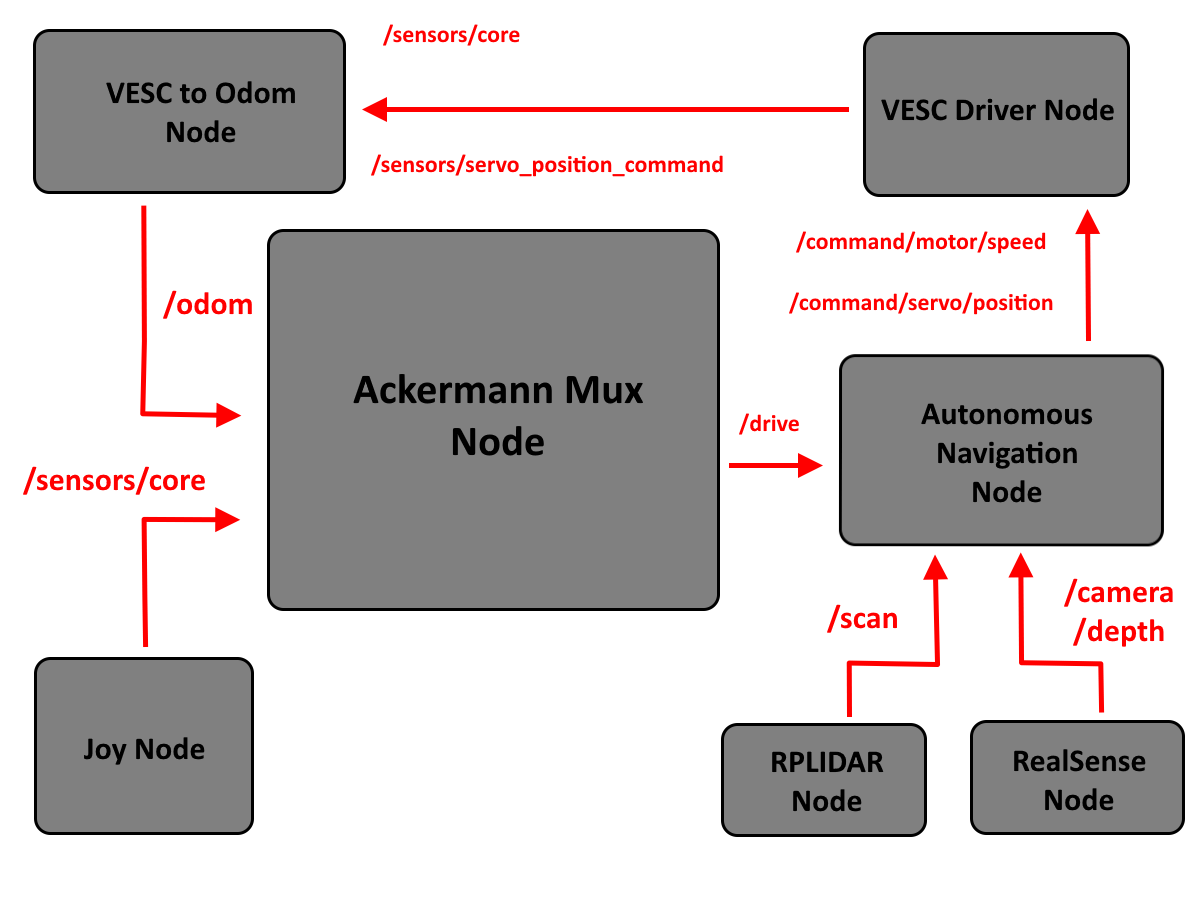
\includegraphics[scale=0.25]{autonomous_architecture.png}
    \caption{Shows software architecture for autonomous navigation in the package.}
    \label{Figure 3}
\end{figure}



In this section, the software architecture of the MacAEV is presented, along with explanations of key algorithms used to fuse the data from the Lidar and stereo camera. 

MacAEV's autonomous navigation software architecture is derived from the University of Pennsylvania's F1Tenth Simulator, an open-source vehicle platform to facilitate driving simulations through ROS. The architecture of this simulator is modified to integrate a navigation node, which publishes ackermann messages to the VESC Motor Controller node when enabled by joystick input. A diagram of the software architecture, illustrating the connections between nodes and topics can be seen in Figure \ref{Figure 3}.







% \subsection{Package Structure}
% This package is a CMake-based and follows the following file structure:


\subsection{Data Fusion}
% 2-D Lidars provide an affordable means of detecting obstacles in the surroundings of the vehicle by mechanically rotating at a high rate and sampling points even faster. 

A key limitation of 2D Lidars is their inablity to detect obstacles below or above their scanning plane. One method of addressing this issue involves the incorporation of a stereo depth camera, and fusing the resulting data obtained from both sensors. This is done through a frame transformation, from the camera's frame of reference to the frame of the Lidar, then comparing the relative distances sampled by both sensors. If the camera depth measurement is less than the Lidar measurement, it indicates that the vehicle is approaching an obstacle below or above the plane of the Lidar scans. In this case, the corresponding lidar scan should be replaced by the camera depth measurement, and the fused ranges are passed in matrix form to the Dual Active Set algorithm. 



%Add Image of diagram



\subsection{Ground Plane Fitting}
% Fusing data obtained from the camera depth and lidar scan returns is done through a comparison of the measurements within the same field of vision. If the camera depth measurement is less than the lidar measurement, it indicates that the vehicle is approaching an obstacle below the plane of the lidar scans.


% Consequently, a replacement is performed before generating the matrices used to solve for the barriers with the data. 
The strategy to fuse lidar and camera data is susceptible to errors, as the camera may inadvertently sample ground points due to misalignment, reflective surfaces and other camera intrinsic parameters which create noise. To mitigate this issue, a ground plane is fitted to a selection of the points within a certain threshold using the Random Sample Consensus (RANSAC) algorithm shown in Algorithm 1. This approach leverages the relatively low height of the MacAEV's camera, as the dominant plane in the image will always be the ground. 

%define variables, explain that hyperparameters must be tuned
%mention that plane filtering must be applied in conjunction with a bandpass filter to eliminate noise for best results

%orientation of camera frame and why
Each iteration of Algorithm 1 samples three valid distinct random points and the coefficients $a,b,c,d$ with $ax + by + cz + d = 0$ satisfying the points are stored. The number of points which satisfy the plane, $num$\textunderscore $pts$ is then compared to $num$\textunderscore $pts$\textunderscore $best$ and the best plane is appropriately updated. This process repeats until either a maximum number of generations $max$\textunderscore $gens$ is reached or $num$\textunderscore $pts$\textunderscore $best$ exceeds a desired number of points which fit the plane, $min$\textunderscore $fit$. 

At each time step, the plane is updated by calling the algorithm and points fitting the plane are omitted from the previously described fusion process. For best results, the hyperparameters $max$\textunderscore $gens$, $min$\textunderscore $fit$, $threshold$ and $height$ require tuning. 



% Experimental trials using the MacAEV car indicated that the filtering worked best in conjunction with an additional bandpass filter to mitigate the influence of noise captured by the depth camera.



% An important remark is that the frame of the depth camera is oriented with increasing y-axis towards the ground, with measurements returned in meters. 


\section{Results (Work In Progress)}

\section{Conclusions and Future Work}
In this article, a data fusion approach to obstacle detection was proposed for the MacAEV, combining measurements obtained from a 2D Lidar and a stereo depth camera. The inherent noise present in the depth camera measurements required additional filtering, which motivated the described RANSAC ground plane approximation algorithm. Using the fused and filtered measurements, an optimization problem was solved, yielding the vectors parametrizing the lines separating obstacles from the vehicle on both sides. These vectors were used in a finite state machine controller to facilitate autonomous navigation. The approach, implemented in C++, worked in real-time as demonstrated by the results.


Overall, this strategy to local planning represents a proposed alternative to laser depth scanning, promising substantial cost savings for both researchers and partners when prototyping self-driving algorithms. Future work will focus on improving both the software and hardware architecture of the system, testing performance in more complex scenarios and feasibility studies of the approach.   

% This approach to obstacle avoidance using lidar-vision sensor fusion and optimization-based navigation reduces the high cost that would ordinarily be associated with investment in a 3-d lidar.    

 
% \section{Ease of Use}

% \subsection{Maintaining the Integrity of the Specifications}

% The IEEEtran class file is used to format your paper and style the text. All margins, 
% column widths, line spaces, and text fonts are prescribed; please do not 
% alter them. You may note peculiarities. For example, the head margin
% measures proportionately more than is customary. This measurement 
% and others are deliberate, using specifications that anticipate your paper 
% as one part of the entire proceedings, and not as an independent document. 
% Please do not revise any of the current designations.

% \section{Prepare Your Paper Before Styling}
% Before you begin to format your paper, first write and save the content as a 
% separate text file. Complete all content and organizational editing before 
% formatting. Please note sections \ref{AA}--\ref{SCM} below for more information on 
% proofreading, spelling and grammar.

% Keep your text and graphic files separate until after the text has been 
% formatted and styled. Do not number text heads---{\LaTeX} will do that 
% for you.

% \subsection{Abbreviations and Acronyms}\label{AA}
% Define abbreviations and acronyms the first time they are used in the text, 
% even after they have been defined in the abstract. Abbreviations such as 
% IEEE, SI, MKS, CGS, ac, dc, and rms do not have to be defined. Do not use 
% abbreviations in the title or heads unless they are unavoidable.

% \subsection{Units}
% \begin{itemize}
% \item Use either SI (MKS) or CGS as primary units. (SI units are encouraged.) English units may be used as secondary units (in parentheses). An exception would be the use of English units as identifiers in trade, such as ``3.5-inch disk drive''.
% \item Avoid combining SI and CGS units, such as current in amperes and magnetic field in oersteds. This often leads to confusion because equations do not balance dimensionally. If you must use mixed units, clearly state the units for each quantity that you use in an equation.
% \item Do not mix complete spellings and abbreviations of units: ``Wb/m\textsuperscript{2}'' or ``webers per square meter'', not ``webers/m\textsuperscript{2}''. Spell out units when they appear in text: ``. . . a few henries'', not ``. . . a few H''.
% \item Use a zero before decimal points: ``0.25'', not ``.25''. Use ``cm\textsuperscript{3}'', not ``cc''.)
% \end{itemize}

% \subsection{Equations}
% Number equations consecutively. To make your 
% equations more compact, you may use the solidus (~/~), the exp function, or 
% appropriate exponents. Italicize Roman symbols for quantities and variables, 
% but not Greek symbols. Use a long dash rather than a hyphen for a minus 
% sign. Punctuate equations with commas or periods when they are part of a 
% sentence, as in:
% \begin{equation}
% a+b=\gamma\label{eq}
% \end{equation}

% Be sure that the 
% symbols in your equation have been defined before or immediately following 
% the equation. Use ``\eqref{eq}'', not ``Eq.~\eqref{eq}'' or ``equation \eqref{eq}'', except at 
% the beginning of a sentence: ``Equation \eqref{eq} is . . .''

% \subsection{\LaTeX-Specific Advice}

% Please use ``soft'' (e.g., \verb|\eqref{Eq}|) cross references instead
% of ``hard'' references (e.g., \verb|(1)|). That will make it possible
% to combine sections, add equations, or change the order of figures or
% citations without having to go through the file line by line.

% Please don't use the \verb|{eqnarray}| equation environment. Use
% \verb|{align}| or \verb|{IEEEeqnarray}| instead. The \verb|{eqnarray}|
% environment leaves unsightly spaces around relation symbols.

% Please note that the \verb|{subequations}| environment in {\LaTeX}
% will increment the main equation counter even when there are no
% equation numbers displayed. If you forget that, you might write an
% article in which the equation numbers skip from (17) to (20), causing
% the copy editors to wonder if you've discovered a new method of
% counting.

% {\BibTeX} does not work by magic. It doesn't get the bibliographic
% data from thin air but from .bib files. If you use {\BibTeX} to produce a
% bibliography you must send the .bib files. 

% {\LaTeX} can't read your mind. If you assign the same label to a
% subsubsection and a table, you might find that Table I has been cross
% referenced as Table IV-B3. 

% {\LaTeX} does not have precognitive abilities. If you put a
% \verb|\label| command before the command that updates the counter it's
% supposed to be using, the label will pick up the last counter to be
% cross referenced instead. In particular, a \verb|\label| command
% should not go before the caption of a figure or a table.

% Do not use \verb|\nonumber| inside the \verb|{array}| environment. It
% will not stop equation numbers inside \verb|{array}| (there won't be
% any anyway) and it might stop a wanted equation number in the
% surrounding equation.

% \subsection{Some Common Mistakes}\label{SCM}
% \begin{itemize}
% \item The word ``data'' is plural, not singular.
% \item The subscript for the permeability of vacuum $\mu_{0}$, and other common scientific constants, is zero with subscript formatting, not a lowercase letter ``o''.
% \item In American English, commas, semicolons, periods, question and exclamation marks are located within quotation marks only when a complete thought or name is cited, such as a title or full quotation. When quotation marks are used, instead of a bold or italic typeface, to highlight a word or phrase, punctuation should appear outside of the quotation marks. A parenthetical phrase or statement at the end of a sentence is punctuated outside of the closing parenthesis (like this). (A parenthetical sentence is punctuated within the parentheses.)
% \item A graph within a graph is an ``inset'', not an ``insert''. The word alternatively is preferred to the word ``alternately'' (unless you really mean something that alternates).
% \item Do not use the word ``essentially'' to mean ``approximately'' or ``effectively''.
% \item In your paper title, if the words ``that uses'' can accurately replace the word ``using'', capitalize the ``u''; if not, keep using lower-cased.
% \item Be aware of the different meanings of the homophones ``affect'' and ``effect'', ``complement'' and ``compliment'', ``discreet'' and ``discrete'', ``principal'' and ``principle''.
% \item Do not confuse ``imply'' and ``infer''.
% \item The prefix ``non'' is not a word; it should be joined to the word it modifies, usually without a hyphen.
% \item There is no period after the ``et'' in the Latin abbreviation ``et al.''.
% \item The abbreviation ``i.e.'' means ``that is'', and the abbreviation ``e.g.'' means ``for example''.
% \end{itemize}
% An excellent style manual for science writers is \cite{b7}.

% \subsection{Authors and Affiliations}
% \textbf{The class file is designed for, but not limited to, six authors.} A 
% minimum of one author is required for all conference articles. Author names 
% should be listed starting from left to right and then moving down to the 
% next line. This is the author sequence that will be used in future citations 
% and by indexing services. Names should not be listed in columns nor group by 
% affiliation. Please keep your affiliations as succinct as possible (for 
% example, do not differentiate among departments of the same organization).

% \subsection{Identify the Headings}
% Headings, or heads, are organizational devices that guide the reader through 
% your paper. There are two types: component heads and text heads.

% Component heads identify the different components of your paper and are not 
% topically subordinate to each other. Examples include Acknowledgments and 
% References and, for these, the correct style to use is ``Heading 5''. Use 
% ``figure caption'' for your Figure captions, and ``table head'' for your 
% table title. Run-in heads, such as ``Abstract'', will require you to apply a 
% style (in this case, italic) in addition to the style provided by the drop 
% down menu to differentiate the head from the text.

% Text heads organize the topics on a relational, hierarchical basis. For 
% example, the paper title is the primary text head because all subsequent 
% material relates and elaborates on this one topic. If there are two or more 
% sub-topics, the next level head (uppercase Roman numerals) should be used 
% and, conversely, if there are not at least two sub-topics, then no subheads 
% should be introduced.

% \subsection{Figures and Tables}
% \paragraph{Positioning Figures and Tables} Place figures and tables at the top and 
% bottom of columns. Avoid placing them in the middle of columns. Large 
% figures and tables may span across both columns. Figure captions should be 
% below the figures; table heads should appear above the tables. Insert 
% figures and tables after they are cited in the text. Use the abbreviation 
% ``Fig.~\ref{fig}'', even at the beginning of a sentence.

% \begin{table}[htbp]
% \caption{Table Type Styles}
% \begin{center}
% \begin{tabular}{|c|c|c|c|}
% \hline
% \textbf{Table}&\multicolumn{3}{|c|}{\textbf{Table Column Head}} \\
% \cline{2-4} 
% \textbf{Head} & \textbf{\textit{Table column subhead}}& \textbf{\textit{Subhead}}& \textbf{\textit{Subhead}} \\
% \hline
% copy& More table copy$^{\mathrm{a}}$& &  \\
% \hline
% \multicolumn{4}{l}{$^{\mathrm{a}}$Sample of a Table footnote.}
% \end{tabular}
% \label{tab1}
% \end{center}
% \end{table}

% \begin{figure}[htbp]
% \centerline{
\includegraphics{fig1.png}}
% \caption{Example of a figure caption.}
% \label{fig}
% \end{figure}

% Figure Labels: Use 8 point Times New Roman for Figure labels. Use words 
% rather than symbols or abbreviations when writing Figure axis labels to 
% avoid confusing the reader. As an example, write the quantity 
% ``Magnetization'', or ``Magnetization, M'', not just ``M''. If including 
% units in the label, present them within parentheses. Do not label axes only 
% with units. In the example, write ``Magnetization (A/m)'' or ``Magnetization 
% \{A[m(1)]\}'', not just ``A/m''. Do not label axes with a ratio of 
% quantities and units. For example, write ``Temperature (K)'', not 
% ``Temperature/K''.

\RestyleAlgo{ruled}

\begin{algorithm}
    \caption{RANSAC Ground Plane Estimation}
        \KwData{Image in OpenCV Format}
        \KwResult{Coefficients $a,b,c,d$ for best fit plane}
    

        gens $\gets 0$\;
        num\textunderscore pts $\gets 0$\;
        max\textunderscore gens $\gets 20$\;
        min\textunderscore fit $\gets 1000$\;
        num\textunderscore pts\textunderscore best $\gets 0$\;
        \While{gens $\leq$ max\textunderscore gens or num\textunderscore pts \textunderscore best $\leq$ min\textunderscore fit} {
            Sample 3 distinct random points in the lower half of image\;
            Compute $a,b,c,d$ for plane containing all three points\;

            \For{row = $0 \dots$ cv\textunderscore sample\textunderscore rows}{

                \For{col = $0 \dots$ cv\textunderscore sample\textunderscore cols}{
                    \If{$(row,col)$ has been sampled to form plane} {
                        continue\;
                    }
                    
                    Deproject pixel at $(row,col)$ using camera instrinsics to find coordinates $x,y,z$\;

                    Compute distance between point and plane\;
                    
                    \If{distance $\leq$ threshold and $y \geq$ height}{ 
                        num\textunderscore pts $\gets$ num\textunderscore pts + 1\;
                    
                    }
                    
                    
                
                }

            
            }

            \If{num\textunderscore pts $\geq$ num\textunderscore pts\textunderscore best}{
                a\textunderscore best $\gets$ a\;
                b\textunderscore best $\gets$ b\;
                c\textunderscore best $\gets$ c\;
                d\textunderscore best $\gets $ d\;
                num\textunderscore pts\textunderscore best $\gets$ num\textunderscore pts\;
            }
            gens $\gets$ gens + 1\;
            
            

            

        }
\end{algorithm}



\section*{Acknowledgment}
The author of this paper extends his gratitude to the National Research Council of Canada for supporting this project through funding, as well as Dr. Shahin Sirouspour and other members of the Telerobotics, Haptics and Computational Vision laboratory for their support.  

% The preferred spelling of the word ``acknowledgment'' in America is without 
% an ``e'' after the ``g''. Avoid the stilted expression ``one of us (R. B. 
% G.) thanks $\ldots$''. Instead, try ``R. B. G. thanks$\ldots$''. Put sponsor 
% acknowledgments in the unnumbered footnote on the first page.

% \section*{References}

% Please number citations consecutively within brackets \cite{b1}. The 
% sentence punctuation follows the bracket \cite{b2}. Refer simply to the reference 
% number, as in \cite{b3}---do not use ``Ref. \cite{b3}'' or ``reference \cite{b3}'' except at 
% the beginning of a sentence: ``Reference \cite{b3} was the first $\ldots$''

% Number footnotes separately in superscripts. Place the actual footnote at 
% the bottom of the column in which it was cited. Do not put footnotes in the 
% abstract or reference list. Use letters for table footnotes.

% Unless there are six authors or more give all authors' names; do not use 
% ``et al.''. Papers that have not been published, even if they have been 
% submitted for publication, should be cited as ``unpublished'' \cite{b4}. Papers 
% that have been accepted for publication should be cited as ``in press'' \cite{b5}. 
% Capitalize only the first word in a paper title, except for proper nouns and 
% element symbols.

% For papers published in translation journals, please give the English 
% citation first, followed by the original foreign-language citation \cite{b6}.

\begin{thebibliography}{00}
% \bibitem{b1} M. Quigley et al., “ROS: An open-source robot operating system,” in Workshops at the IEEE International Conference on Robotics and Automation, 2009.

% \bibitem{b2} S. Macenski, T. Foote, B. P. Gerkey, C. Lalancette, and W. Woodall, “Robot Operating System 2: Design, Architecture, and Uses In The Wild.,” CoRR, vol. abs/2211.07752, 2022.

\bibitem{b1} Susnea, I., Minzu, V., Vasiliu, G.: Simple, real-time obstacle avoidance algorithm for mobile robots. In: International Conference on Computational
intelligence, man-machine systems and cybernetics. World Scientific, Engineering Academy and Society. pp. 24–29. WESEAS’09 (2009)

\bibitem{b2} D. Li, P. Auerbach, and O. Okhrin, “Towards Autonomous Driving with Small-Scale Cars: A Survey of Recent Development.,” CoRR, vol. abs/2404.06229, 2024.


\bibitem{b3} S. Badrloo, M. Varshosaz, S. Pirasteh, and J. Li, “Image-Based Obstacle Detection Methods for the Safe Navigation of Unmanned Vehicles: A Review.,” Remote. Sens., vol. 14, no. 15, p. 3824, 2022.

\bibitem{b4} V. Sezer and M. Gokasan, “A novel obstacle avoidance algorithm: ‘Follow the Gap Method’.,” Robotics Auton. Syst., vol. 60, no. 9, pp. 1123–1134, 2012.

\bibitem{b5} “Jetson AGX Orin developer KIT User Guide,” NVIDIA Developer, https://developer.nvidia.com/embedded/learn/jetson-agx-orin-devkit-user-guide/index.html 


\bibitem{b6} RPLIDAR A2 Low Cost 360 Degree Laser Range Scanner, https://www.slamtec.ai/wp-content/uploads/2023/11/LD310 \textunderscore SLAMTEC \textunderscore rplidar \textunderscore datasheet \textunderscore A2M12\textunderscore v1.0 \textunderscore en.pdf 


\bibitem{b7} A. Grunnet-Jepson et al., “Intel-Realsense D400 Series Datasheet,” Intel RealSense Technology


%https://www.intel.com/content/dam/support/us/en/documents/emerging-technologies/intel-realsense-technology/Intel-RealSense-D400-Series-Datasheet.pdf 

\bibitem{b8} D. Goldfarb and A. Idnani, “A numerically stable dual method for solving strictly convex quadratic programs,” Sep. 1983, doi: 10.1007/bf02591962.



\end{thebibliography}
\vspace{12pt}
\color{red}
% IEEE conference templates contain guidance text for composing and formatting conference papers. Please ensure that all template text is removed from your conference paper prior to submission to the conference. Failure to remove the template text from your paper may result in your paper not being published.

\end{document}
